\documentclass[a4paper]{article}

\usepackage[utf8]{inputenc}
\usepackage{amssymb, amsfonts, latexsym, amsthm, amsmath, framed}
\usepackage{esvect}
\usepackage{parskip}

\usepackage{amsmath, amssymb, framed, tcolorbox}
\tcbuselibrary{theorems}

\usepackage{graphicx}

\usepackage{mathrsfs}

\usepackage{xcolor}

\usepackage[colorlinks,linkcolor=blue,citecolor=blue,urlcolor=blue]{hyperref} % 

%% Bibliography support
\usepackage[backend=bibtex,isbn=false,url=false]{biblatex} 


\addbibresource{ref.bib}

\newcommand{\ba}{\backslash}
\newcommand{\Q}{\mathbb{Q}}
\newcommand{\C}{\mathbb{C}}
\newcommand{\R}{\mathbb{R}}
\newcommand{\N}{\mathbb{N}}
\newcommand{\Z}{\mathbb{Z}}
\newcommand{\F}{\mathbb{F}}
\newcommand{\rank}{\text{rank}}
\newcommand{\slC}{\mathfrak{sl}_3\mathbb{C}}
% figure support
\usepackage{import}
\usepackage{xifthen}
\pdfminorversion=7
\usepackage{pdfpages}
\usepackage{transparent}
\newcommand{\incfig}[1]{%
	\def\svgwidth{\columnwidth}
	\import{./figures/}{#1.pdf_tex}
}

\newtheoremstyle{bfnote}%
  {}{}
  {}{}
  {\bfseries}{.}
  { }{\thmname{#1}\thmnumber{ #2}\thmnote{ (#3)}}

\theoremstyle{bfnote} % set the style for the following theorems

\newtheorem{thm}{Theorem}[section] %\newtheorem{name}{display-text}[numbered-within]

\newtheorem{lem}[thm]{Lemma} %\newtheorem{name}[numbered-like]{display-text}
\newtheorem{cor}[thm]{Corollary}
\newtheorem{prop}[thm]{Proposition}
\newtheorem{alg}[thm]{Algorithm}

\theoremstyle{bfnote}                  % switch to a different style
\newtheorem{defn}[thm]{Definition}
\newtheorem{conj}[thm]{Conjecture}


\theoremstyle{example}                       % another style
\newtheorem{prob}[thm]{Problem}


\theoremstyle{remark}                       % another style
\newtheorem{exmp}[thm]{Example}  % (note:the "example" style is not really good for long examples-- typesets them in italics!)
\newtheorem{rem}[thm]{Remark}
\newtheorem{claim}[thm]{Claim}
\renewcommand{\theclaim}{}

%% If you use numbered equations in a long document, it is preferred to number
% as (x.y), where x is section number, y is equation number

\numberwithin{equation}{section}




\pdfsuppresswarningpagegroup=1

\usepackage{tcolorbox}
\usepackage{tikz}
\tcbuselibrary{theorems, skins, breakable}

\title{Decomposition of Adjoint Representation, $\slC$}
\date{Spring 2022, Algebra 2}
\author{Yuxuan Sun}


\begin{document}

\maketitle
\tableofcontents

\section{Introduction}
This paper aims to give an introduction on Lie algebra and representations, specifically the adjoint representation. It will start with some basic usage of linear algebra, then introduce a way to decompose the adjoint representation and how we could use the result of decompositions to study the actions of other elements in our Lie algebra.

\section{Lie Algebra}
My curiosity before this paper is to study something geometric, and that's when Lie groups naturally appeared in my search, as they provide a way to express geometric objects, and to do differentiation, Lie algebra is useful. To study Lie algebra, we could borrow representations. This paper will not talk about Lie group: this paragraph is for motivations if one wonders.

\begin{defn}[bracket and Lie algebra, \cite{humph}]\label{bracket}
	A vector space $\mathfrak{g}$ over a field $F$, with an operation $\left[ \cdot, \cdot \right] $ from $\mathfrak{g} \times \mathfrak{g} \to  \mathfrak{g}$, called the  \textbf{bracket} or \textbf{commutator} of $x$ and  $y$, is called a  \textbf{Lie algebra} over $F$ if the following properties are satisfied:
\begin{enumerate}
		 \item The bracket operation is bilinear, i.e.
\begin{enumerate}
	\item $[x,y_1+y_2] = [x,y_1] + [x,y_2]$ and $[x_1+x_2,y] = [x_1,y] + [x_2,y]$, for all $x, x_1, x_2, y, y_1,y_2 \in \mathfrak{g}$.
	\item $[\lambda x, y] = \lambda[x,y] = [x, \lambda y]$, for all $\lambda \in F$ and $x, y \in \mathfrak{g}$.
\end{enumerate}
		 \item $[x,x] = 0$, for all $x \in \mathfrak{g}$.
		 \item $[x,[y,z]]+[y,[z,x]] +[z,[x,y]] = 0$, for all $x,y,z \in \mathfrak{g}$.
	\end{enumerate}
\end{defn}

\bigskip

\begin{thm}[anti-commutativity of bracket]\label{anti-commutativity}
	Given a Lie algebra $\mathfrak{g}$ equipped with a bracket operation,for all  $x,y \in \mathfrak{g}$, we always have $[x,y] = -[y,x]$, indicating the \textbf{anti-commutativity of bracket} on $\mathfrak{g}$. 	
\end{thm}

\begin{proof}
Given any $x,y \in \mathfrak{g}$, using the properties we defined above, we could have:
\begin{align*}
	0 &= [x+y, x+y] & \textbf{property 2} \\
	 &= [x, x+y] + [y, x+y] & \textbf{property 1a} \\
		   &= [x,x] + [x,y] + [y,x] + [y,y] & \textbf{property 1a} \\
		   &= [x,y] + [y,x] & \textbf{property 2} \\
	[x,y] &= -[y,x]
\end{align*}
\end{proof}
Thus intuitively, the bracket operation measures ``how commutative $x$ and  $y$ are''. For example, if $x, y$ are commutative under the bracket operation,  i.e. if  $[x,y] = [y,x]$, then  $[x,y]$ should immediately give me  $0$ for Theorem \ref{anti-commutativity} to hold. 

\section{Decomposition of the Adjoint Representation of $\mathfrak{sl}_3\C$}
In this section, we are going to look at the adjoint representation of $\mathfrak{sl}_3\C$ and see how it could be decomposed into eigenspaces of a special subspace of  $\mathfrak{sl}_3\C$. This is a special case of a more general statement which would be mentioned at the end of the paper.

\subsection{Preliminary}
Before everything, let's look at what  $\mathfrak{sl}_3\C$ is.
\bigskip
\begin{exmp}[$\mathfrak{sl}_3\C$, \cite{hall}]\label{exmp:sl3}
	The Lie algebra $\mathfrak{sl}_3\C$ is a vector space of  $3 \times 3$ matrices with trace  $0$ over  $\C$. In other words \[
		\mathfrak{sl}_{3}\C = \left\{ \begin{bmatrix} a & c & d \\
		e & -a+b & f \\ g & h & -b\end{bmatrix} \mid a,b,c,d,e,f,g,h \in \C \right\} 
	.\]
	We could see that $\mathfrak{sl}_3\C$ is an  $8$-dimensional vector space with the following basis: \[
	\mathcal{B}_{\mathfrak{sl}_{3}} = \left\{ H_1 = \begin{bmatrix} 1 & 0 &0 \\ 0 & -1 & 0 \\ 0 &0 &0 \end{bmatrix}, H_2 = \begin{bmatrix} 0 &0 &0 \\ 0 &1&0 \\ 0&0&-1 \end{bmatrix}   \right\} \bigcup \left\{ E_{i,j} \mid i \neq j, 1\le i,j \le 3\right\}. 
\] $E_{i,j}$ is a matrix where ${E_{i,j}}_{ij} = 1$ and other places are $0$, for example:\[
		E_{1,3} = \begin{bmatrix} 0 & 0 & 1 \\ 0 & 0 &0 \\ 0 &0 &0 \end{bmatrix}. 
	\] 
\end{exmp}

To use representation, we could define one on $\mathfrak{sl}_3\C$ just using the bracket operation, namely as     the following.
\begin{defn}[adjoint representation of $\mathfrak{sl}_3\C$]\label{adjoint}
	Give $X \in \mathfrak{sl}_3\C$, define a linear map $\operatorname{ad}_X : \mathfrak{sl}_3\C \to \mathfrak{sl}_3\C$ as: \[
		\operatorname{ad}_X(Y) = [X,Y]
	\] the map $X \mapsto \operatorname{ad}_X$ is called an \textbf{adjoint representation} of $\mathfrak{sl}_3\C$.
\end{defn}
\begin{rem}[$\mathfrak{h} \subset \mathfrak{sl}_{3}\C$]
	Denote $\mathfrak{h}$ as the two dimensional subspace of all diagonal matrices in  $\mathfrak{sl}_3\C$. Namely:  \[
		\mathfrak{h} = \operatorname{Span}\left\{ H_1=\begin{bmatrix} 1 & 0 &0 \\ 0 & -1 & 0 \\ 0 &0 &0 \end{bmatrix}, H_2 = \begin{bmatrix} 0 &0 &0 \\ 0 &1&0\\0&0&-1 \end{bmatrix}   \right\} 
	\] 
\end{rem}

\bigskip

The usage of linear functional will appear later, and the definition is here for future reference.
\begin{defn}[linear functional]\label{linearFunctional}
	A linear functional $T$ on a complex vector space  $V$ is a function  $T: V \to \C$ which satisfies the following properties:
	\begin{enumerate}
		\item $T(v+w) = T(v) + T(w)$ 
		\item $T(\alpha v) = \alpha T(v)$
	\end{enumerate}
\end{defn}

Now we've chosen our special subspace $\mathfrak{h} \subset \mathfrak{sl}_3\C$, let's look at what it means to be an eigenvector, eigenvalue, and eigenspace for $\mathfrak{h}$.
\subsection{Decomposition Using Eigenspaces}

\begin{defn}[eigenvector and eigenvalue for a vector space, \cite{fulton}]
	Let $\mathfrak{h}$ be a subspace of a vector space $V$, an  \textbf{eigenvector} for $\mathfrak{h}$ refers to a vector  $v$ that is an eigenvector for all  $H \in \mathfrak{h}$, in other words: \[
		H v = \alpha(H) v \quad \text{for all $H \in \mathfrak{h}$},
	\]  where $\alpha$ is a linear functional on  $H$, and we call $\alpha$ as an \textbf{eigenvalue}. 
\end{defn}

\begin{defn}[eigenspace for the adjoint action of $\mathfrak{h}$ on  $\mathfrak{sl}_3\C$,\cite{fulton}]
	 Give $\mathfrak{h} \subset \mathfrak{sl}_3\C$ as we defined above, an eigenspace of $\mathfrak{h}$ with a linear functionl  $\alpha$ as an eigenvalue, denoted as  $\mathfrak{g}_{\alpha}$, contains all $M \in \mathfrak{sl}_3\C$ such that \[
		 \left[ H,M \right] = \operatorname{ad}_{H}(M) = HM - MH = \alpha(H) \dot M. 
	 \] 
\end{defn}

\bigskip

It's still a bit fuzzy: we don't know what our linear functionals (eigenvalues) are and we also don't know what our $M$ (eigenvectors) look at. Thus let's spell everything out explicitly.

Take any  $H \in \mathfrak{h}$ and any $M \in \mathfrak{sl}_3\C$, namely: \[
		H = \def\a{\color{red}a} \begin{bmatrix} \a_1 & 0 & 0 \\ 0 & \a_2 &0 \\ 0 &0 &\a_3 \end{bmatrix}, M = \def\m{\color{blue}m} \begin{bmatrix} \m_{11} & \m_{12} & \m_{13} \\ \m_{21} & \m_{22} & \m_{23} \\ \m_{31} & \m_{32} & \m_{33} \end{bmatrix} 
	\]
Let's see what the adjoint $\operatorname{ad}_{H}(M)$ give us.
\begin{align*}
[H,M] &= HM - MH \\ &= \def\a{\color{red}a} \def\m{\color{blue}m} \begin{bmatrix} \color{red}{(}\a_1-\a_1)\m_{11} & \color{red}{(}\a_1-\a_2)\m_{12} & \color{red}{(}\a_1-\a_3)\m_{13} \\ \color{red}{(}\a_2-\a_1)\m_{21} & \color{red}{(}\a_2-\a_2)\m_{22} & \color{red}{(}\a_2-\a_3)\m_{23} \\ \color{red}{(}\a_3-\a_1)\m_{31} & \color{red}{(}\a_3-\a_2)\m_{32} & \color{red}{(}\a_3-\a_3)\m_{33} \end{bmatrix} \\
		      &=  \def\a{\color{red}a} \def\m{\color{blue}m} \begin{bmatrix} 0 \cdot \m_{11} & \color{red}{(}\a_1-\a_2)\m_{12} & \color{red}{(}\a_1-\a_3)\m_{13} \\ \color{red}{(}\a_2-\a_1)\m_{21} & 0 \cdot \m_{22} & \color{red}{(}\a_2-\a_3)\m_{23} \\ \color{red}{(}\a_3-\a_1)\m_{31} & \color{red}{(}\a_3-\a_2)\m_{32} & 0 \cdot \m_{33} \end{bmatrix} 
\end{align*}

If we want $M$ to be an eigenvalue under the adjoin action, then by definition, for all  $H \in \mathfrak{h}$, and given a linear functional $\alpha$, we would want: \[
	\def\a{\color{red}a} \def\m{\color{blue}m} \begin{bmatrix} 0 \cdot \m_{11} & \color{red}{(}\a_1-\a_2)\m_{12} & \color{red}{(}\a_1-\a_3)\m_{13} \\ \color{red}{(}\a_2-\a_1)\m_{21} & 0 \cdot \m_{22} & \color{red}{(}\a_2-\a_3)\m_{23} \\ \color{red}{(}\a_3-\a_1)\m_{31} & \color{red}{(}\a_3-\a_2)\m_{32} & 0 \cdot \m_{33} \end{bmatrix} = \alpha(H) \begin{bmatrix} \m_{11} & \m_{12} & \m_{13} \\ \m_{21} & \m_{22} & \m_{23} \\ \m_{31} & \m_{32} & \m_{33} \end{bmatrix}  
\] 

An immediate observation is that all diagonal matrices are eigenvectors of $\mathfrak{h}$ with eigenvalue  $0$. In other words,  $\mathfrak{h}$ is an eigenspace  of itself with eigenvalue $0$.

(If one wants to be more rigorous, by eigenvalue  $0$, we mean a linear functional that sends everything to $0$, so it's a  $T: \mathfrak{h}\to \C$ such that $H \mapsto 0$. )

Another important observation is that, we could only have $6$ eigenvalues for each  $H \in \mathfrak{h}$: $a_1-a_2, a_1-a_3, a_2-a_3, a_2-a_1, a_3-a_1, a_3-a_2$. Because we want our eigenvalue to be applicable for all $H \in \mathfrak{h}$, whose only constraint is $a_1+a_2+a_3 = 0$, we could only afford to hold them separately as eigenvalue.

In more details, suppose we have  $M = \begin{bmatrix} 0 & 1 & 0 \\ 0 & 0 & 1 \\ 0 & 0 &0  \end{bmatrix} $, this matrix could not be an eigenvector, because if so, it would require $a_1 - a_2 = a_2 - a_3$, but this constrain cannot be found on all matrices $H \in \mathfrak{h}$. Thus all our eigenvecotrs (besides diagonal matrices as we talked before) could only have one $1$  and other places being zero.

The conclusion of our observations above is that each eigenspace $\mathfrak{g}_{\alpha}$ could be generated by a $E_{i,j} \in \mathcal{B}_{{\mathfrak{sl}_3}}$, as introduced in Example \ref{exmp:sl3}, where $i \neq j$ and $E_{ij} = 1$ and other places zero.

\bigskip

Let's them formally define our linear functional: 
\begin{defn}[$L_i$]
	Let $L_i: \mathfrak{h} \to \C$ be a linear functional such that \[
		L_i \left(\begin{bmatrix} a_1 & 0 &0 \\ 0 & a_2 & 0 \\ 0 &0 &a_3 \end{bmatrix}\right) = a_i
	\] it satisfies the requirement of a linear functional, the proof is omitted:

	$L_i(A+B) = L_i(A) + L_i(B), L_i(aA) = aL_i(A)$.
\end{defn}
One shall see this as a natural and simple derivation from the discussion above, as all our linear functionls do is to ``fetch'' the $a_1, a_2, a_3$ from all  $H \in \mathfrak{h}$ for us. 

Together, we could have an overview for our eigenvalues.

\begin{rem}[$\mathfrak{h}^*$, eigenvalues of  $\mathfrak{h}$] 
	Denote $\mathfrak{h}^*$ as the set of all eigenvalues of  $\mathfrak{h}$, we'll have:  \[
		\mathfrak{h}^* = \left\{ L_i - L_j \mid 1\le  i,j \le 3\right\} 
	\] 
\end{rem}
Recall the conclusion of our observations above, we know that $\mathfrak{g}_{L_i-L_j}$ will be generated by the element $E_{i,j} \in \mathcal{B}_{\mathfrak{sl}_3}$.

Now we have a formal way to decompose $\mathfrak{sl}_3$ under the adjoint representation:  \begin{equation}
	\mathfrak{sl}_3\C = \mathfrak{h} \oplus \left( \oplus \mathfrak{g}_{\alpha} \right) 
\end{equation}  where $\alpha$ ranges over  $\mathfrak{h}^*$.

\subsection{The Action of Other Elements in $\mathfrak{sl}_3$}

The major takeaway from the decomposition is that now we have a clearer way to look at $\mathfrak{sl}_3\C$: it is not only a bunch of trace  $0$ matrices but also a direct sum of all the eigenspaces of  $\mathfrak{h}$ under the adjoint representation.

Therefore, given any matrix in  $\mathfrak{sl}_3$, if we want to know how it acts on  $\mathfrak{sl}_3$ under the adjoint action, we could just look at what it does on each eigenspace of  $\mathfrak{h}$. This new perspective, as we'll see, is quite simple and direct.

First let's not take any arbitrary matrix, but choose our old friend $H \in \mathfrak{h}$, and put the eigenspaces into a figure.

\begin{figure}[h!]
 \centering
 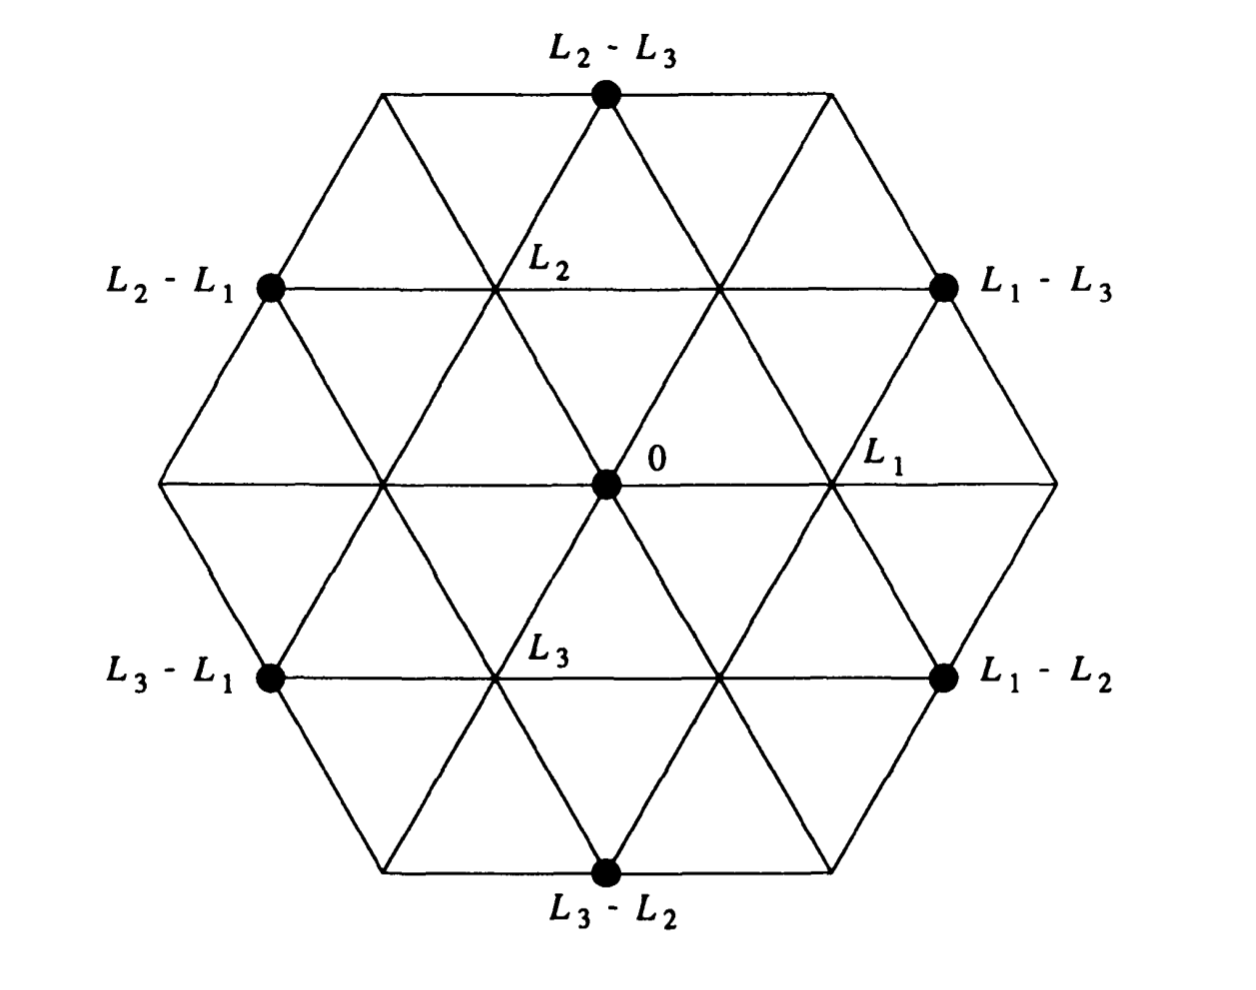
\includegraphics[width=3 in]{eigenvalue}
 \caption{eigenspaces denoted by eigenvalues of $\mathfrak{h}$}
 \label{eigenvalue}
 \end{figure}

 In Figure \ref{eigenvalue}, all the solid dots represent our eigenvalues. Beyond that, this graph also tells us how $\mathfrak{h}$ acts on $\mathfrak{sl}_3$: given any subspace  $\mathfrak{g}_{L_i-L_j}$, $\mathfrak{h}$ send it to itself, since all the elements in the subspace is an eigenvector of  $\mathfrak{h}$.
\bigskip

Now let's look at the rest of $\slC$. We would need to rely on the properties of bracket in Definition \ref{bracket}.

Take any $X \in \mathfrak{g}_\alpha$, and any $Y \in \mathfrak{g}_{\beta}$, we would like to know how $X$ acts on  $Y$ under the adjoin action, i.e. where would $\left[ X,Y \right] $ be? 

We could know that by looking at how  $\mathfrak{h}$ would act on  $\left[ X,Y \right] $. Take any $H \in \mathfrak{h}$, we could have:
\begin{align*}
	[H, [X,Y]] &=  -[X,[Y,H]] - [Y,[H,X]] & \text{property 3} \\
	  &= [X,-[Y,H]] - [Y, [H,X]] & \text{property 2b} \\
		  &= [X, [H,Y]] + [[H,X],Y] & \text{Theorem } \ref{anti-commutativity} \\
		  &= [X, \beta(H) Y] + [\alpha(H)X, Y] & \text{$X,Y$ with eigenvalues  $\alpha, \beta$} \\
		  &= \beta(H)[X,Y] + \alpha(H)[X,Y] & \text{property 2b} \\
		  &= \left( \alpha(H) + \beta(H) \right)[X,Y]  
\end{align*}

From the above deduction, we know that $[X,Y]$ is an eigenvector of  $\mathfrak{h}$, whose eigenvalue is  $\alpha + \beta$. Since  $X, Y$ are arbitrarily chosen from  $\mathfrak{h}_\alpha, \mathfrak{h}_\beta$, we now know how would one eigenspace act on another under the adjoint representation, namely:  \begin{equation}\label{other}
	\operatorname{ad}\left( \mathfrak{g}_{\alpha} \right): \mathfrak{g}_{\beta} \to \mathfrak{g}_{\alpha+\beta} 
\end{equation}

We could see it more directly on an exciting figure.

\begin{figure}[h!]
 \centering
 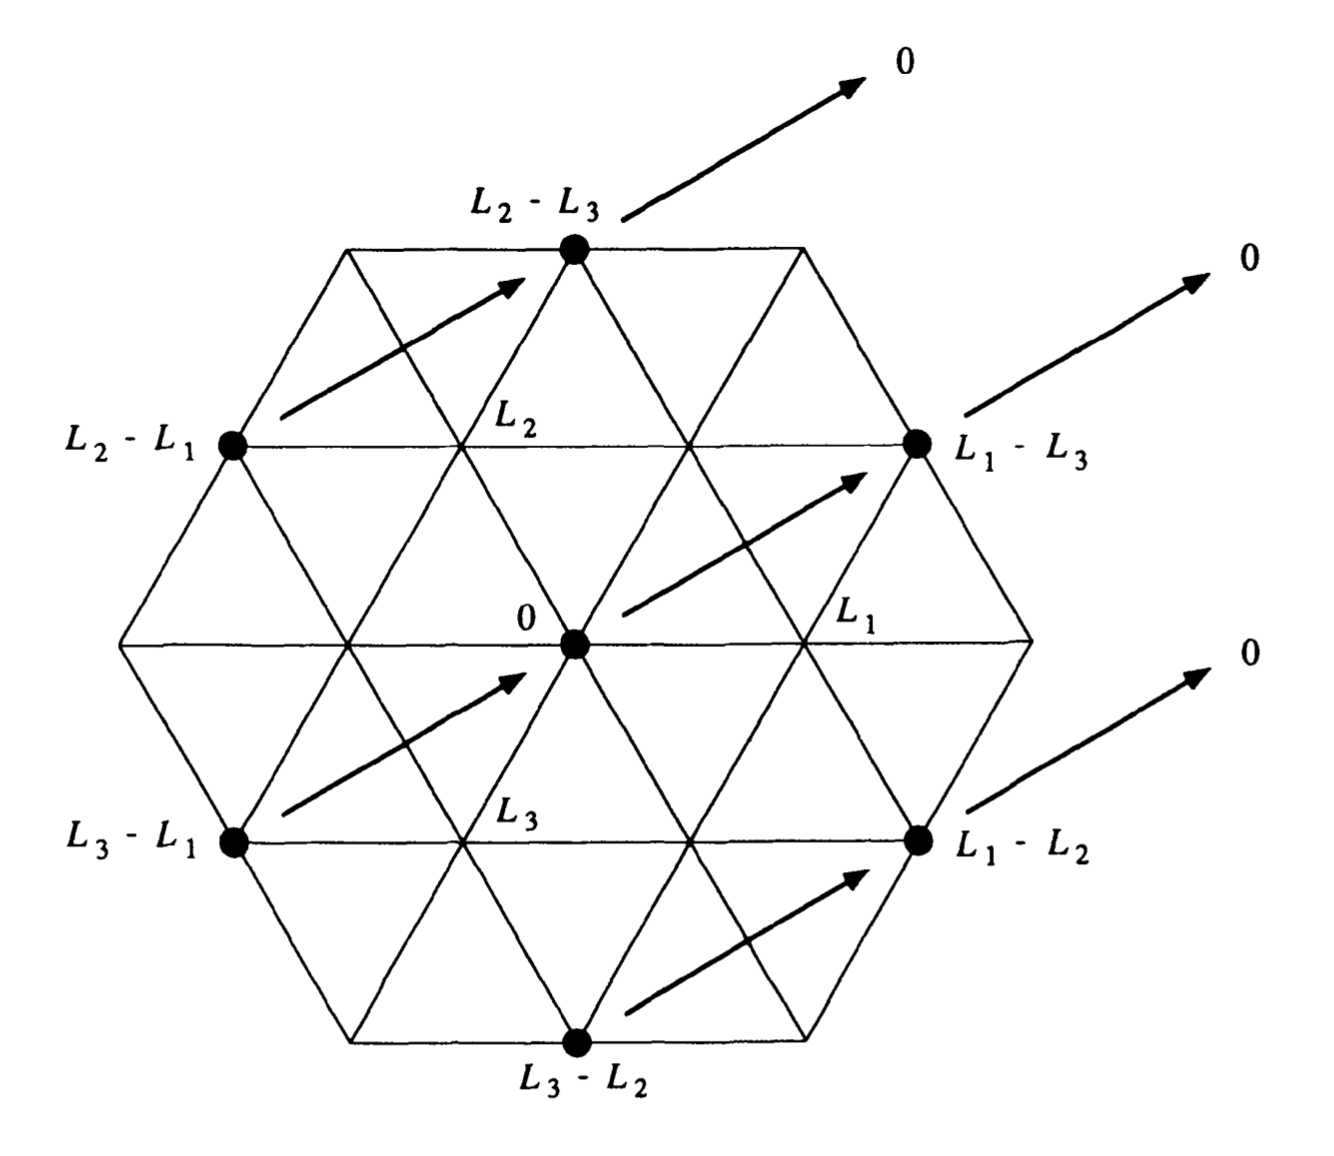
\includegraphics[width=4 in]{L1-L3}
 \caption{How $\mathfrak{g}_{L_1-L_3}$ acts on other eigenspaces, \cite{fulton}}
 \label{L1-L3}
 \end{figure}

 In Figure \ref{L1-L3}, give any eigenspace $\mathfrak{g}_{\beta}$, we use arrows to indicate how  $\mathfrak{g}_{L_1-L_3}$ would act on $\mathfrak{g}_\beta$. Based on Equation \ref{other}, if we take for example $\mathfrak{g}_{L_2-L_1}$, we know the eigenvalue of the destination is $L_1-L_3 + L_2 - L_1 = L_2 - L_3$, as indicated by the arrow.

\section{Conclusion and Future Study}

Decomposition is nice! Besides Maschke we saw in class, now we see another way to decompose representations -- via eigenspaces. If we choose a subspace that ``behaves nicely'' as the diagonal matrices we saw here, we would be able to study how other stuff act on each other by just looking at the eigenspaces of the nice subspace.

There are so many more to be explored. For example, what more could we play with the figures? How would irreducibility influence our eigenvalues? Is there any other way to decompose the space using eigenvalues of a maybe less nice subspace? 

At the end, I want to thank my advisors Elizabeth Milićević and David Lippel when they bear with me when I kept switching topics of this paper and supported and helped me when I had any question. I would probably never even decided what I wanted to write without their help, and if anyone besides them would read this, I hope this would lay out some foundations for Lie algebra and representation theory.

\newpage
\printbibliography
\end{document}










